\begin{frame}[fragile]
\frametitle{The Expression Problem}
\begin{block}{Cheat Detection}
lichess.org is an open-source chess server, written using Scala.
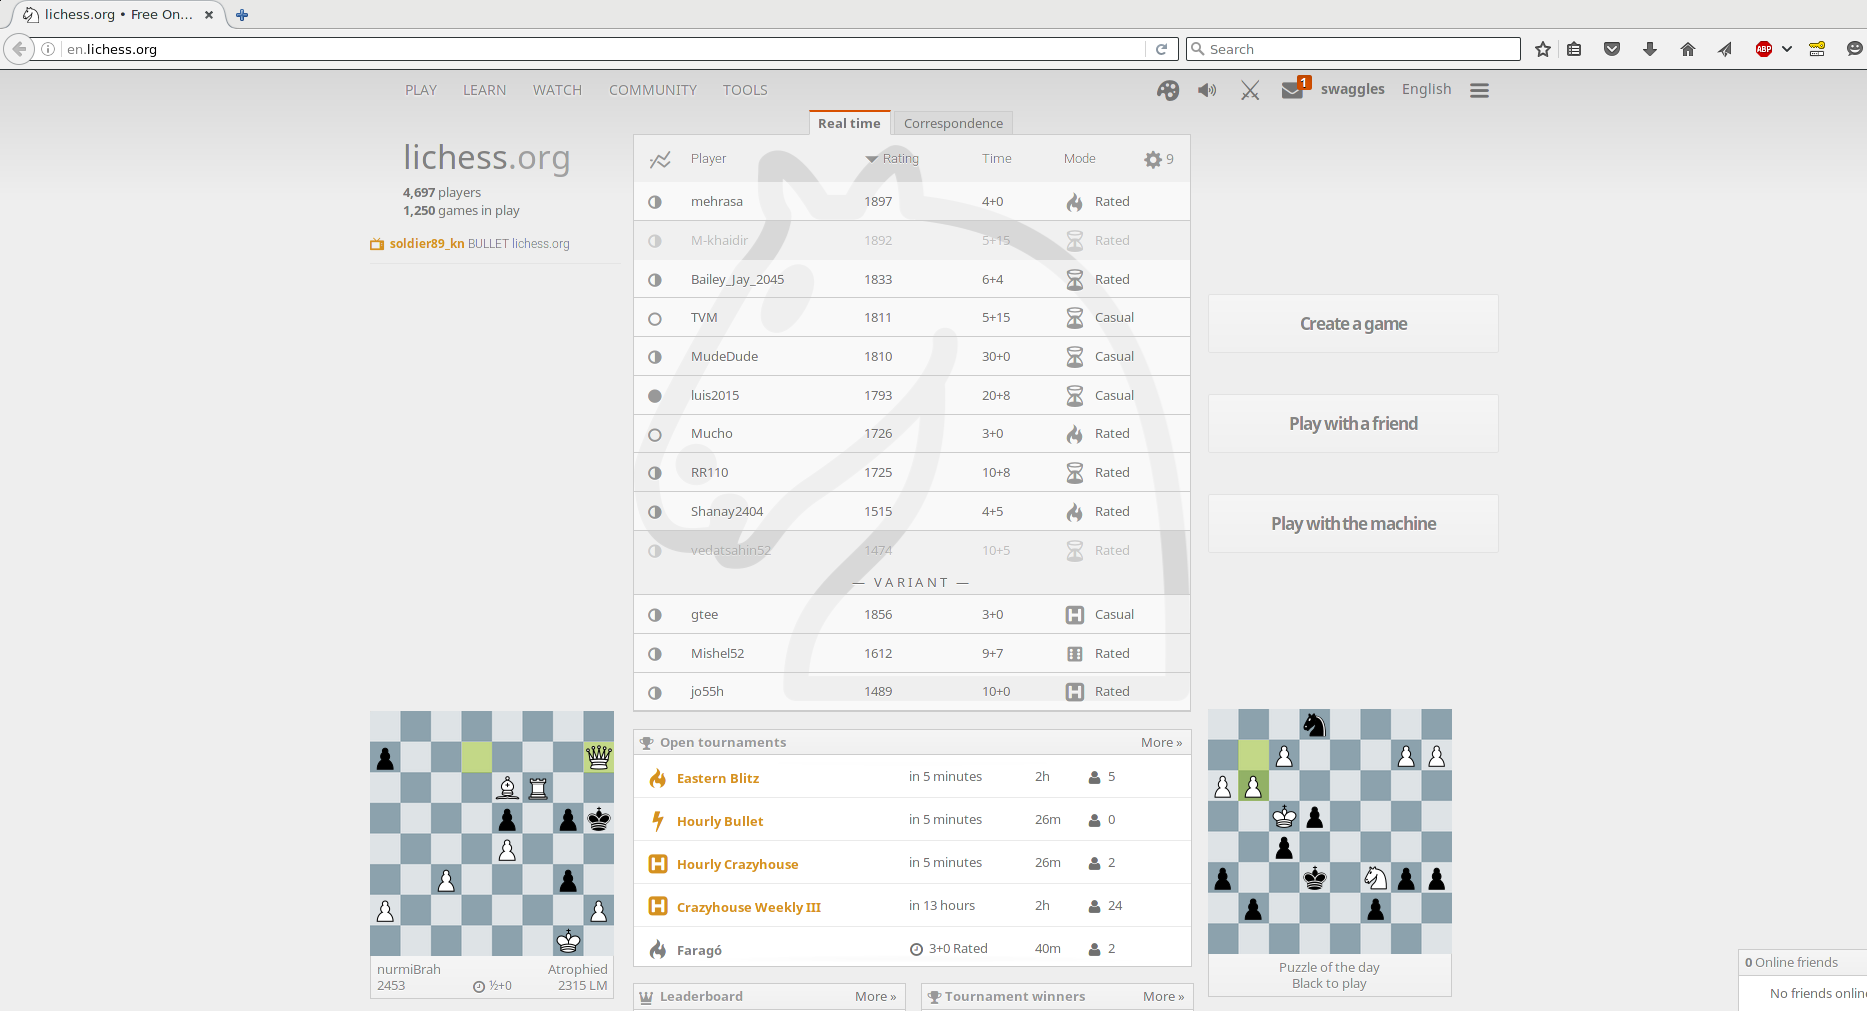
\includegraphics[height=0.4\textheight,natwidth=1867,natheight=1011]{image/lichess.png}
\end{block}
\end{frame}

\begin{frame}[fragile]
\frametitle{The Expression Problem}
\begin{block}{Cheat Detection}
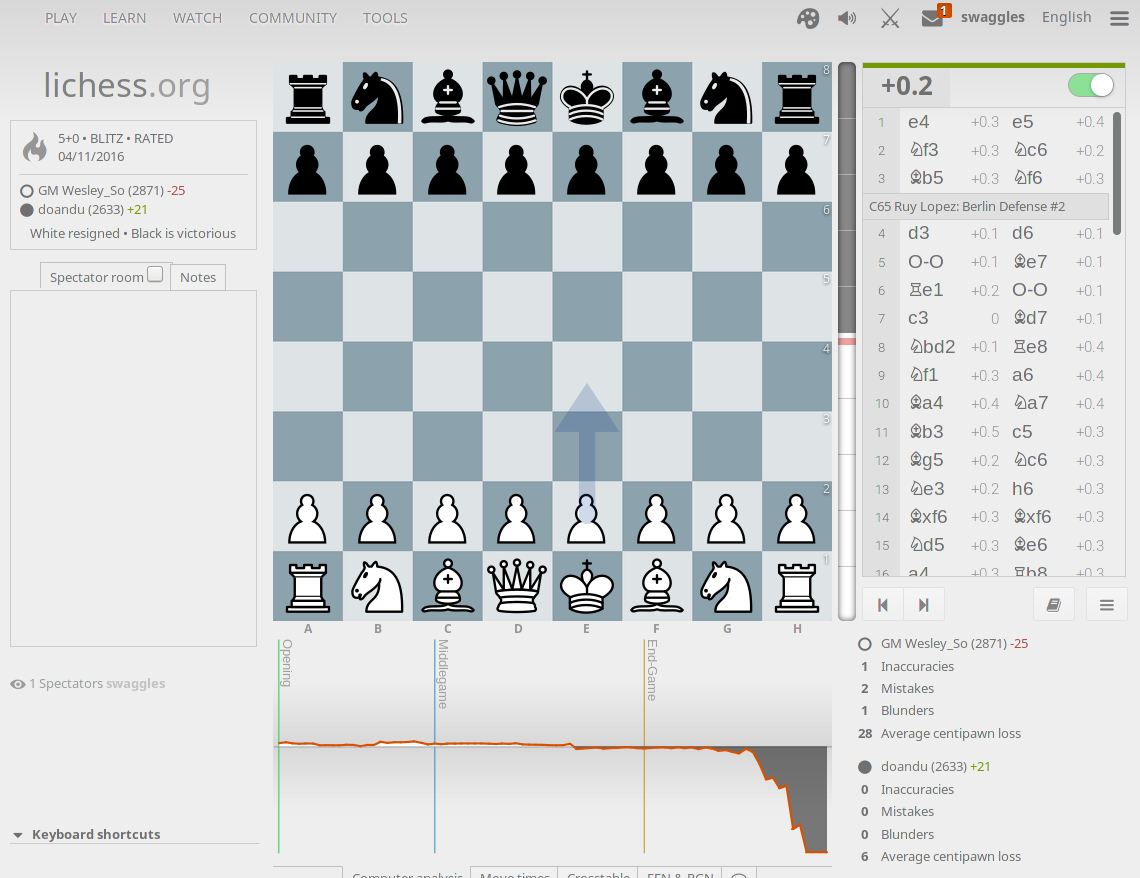
\includegraphics[height=0.5\textheight,natwidth=1140,natheight=878]{image/lichess-wesley-so.png}
\par
Here is the world \#12 being beaten by a patzer using computer-assistance.
\end{block}
\end{frame}

\begin{frame}[fragile]
\frametitle{The Expression Problem}
\begin{block}{Cheat Detection}

\includegraphics[height=0.2\textheight,natwidth=883,natheight=184]{image/lichess-wesley-so-announce.png}
\par
Here is the world \#12 being beaten by a patzer using computer-assistance.
\end{block}
\end{frame}
